\chapter{Diseño e implementación} % Main chapter title
\label{Chapter3} % Change X to a consecutive number; for referencing this chapter elsewhere, use \ref{ChapterX}

En este capítulo se abordan cuestiones de diseño, se presentan los requerimientos del sistema y la solución propuesta. Se detalla la solución en términos de arquitectura, patrones de software, descripción de componentes e implementación. En el desarrollo se utiliza la plataforma de hardware EDU-CIAA\citep{CIAA}, la API Firmware\_ v3\citep{firmwarev3}, y freeRTOS\citep{freeRTOS} como sistema operativo de tiempo real.\\

% Siguiendo lineamientos de ingeniería de software, se presentan los requerimientos, funcionalidades y casos de uso como ejes principales del espacio problema. Luego se presenta la arquitectura, la organización del código fuente, los patrones implementados, diagramas de secuencia y diagramas de interacción entre componentes como detalle del espacio solución.\\


\definecolor{mygreen}{rgb}{0,0.6,0}
\definecolor{mygray}{rgb}{0.95,0.95,0.95}
\definecolor{mygray50}{rgb}{0.5,0.5,0.5}
\definecolor{mymauve}{rgb}{0.58,0,0.82}

%%%%%%%%%%%%%%%%%%%%%%%%%%%%%%%%%%%%%%%%%%%%%%%%%%%%%%%%%%%%%%%%%%%%%%%%%%%%%
% parámetros para configurar el formato del código en los entornos lstlisting
%%%%%%%%%%%%%%%%%%%%%%%%%%%%%%%%%%%%%%%%%%%%%%%%%%%%%%%%%%%%%%%%%%%%%%%%%%%%%
\lstset{ %
  backgroundcolor=\color{mygray},   % choose the background color; you must add \usepackage{color} or \usepackage{xcolor}
  basicstyle=\footnotesize,        % the size of the fonts that are used for the code
  breakatwhitespace=false,         % sets if automatic breaks should only happen at whitespace
  breaklines=true,                 % sets automatic line breaking
  captionpos=b,                    % sets the caption-position to bottom
  commentstyle=\color{mygreen},    % comment style
  deletekeywords={...},            % if you want to delete keywords from the given language
  %escapeinside={\%*}{*)},          % if you want to add LaTeX within your code
  %extendedchars=true,              % lets you use non-ASCII characters; for 8-bits encodings only, does not work with UTF-8
  %frame=single,	                % adds a frame around the code
  keepspaces=true,                 % keeps spaces in text, useful for keeping indentation of code (possibly needs columns=flexible)
  keywordstyle=\color{blue},       % keyword style
  language=[ANSI]C,                % the language of the code
  %otherkeywords={*,...},           % if you want to add more keywords to the set
  numbers=left,                    % where to put the line-numbers; possible values are (none, left, right)
  numbersep=5pt,                   % how far the line-numbers are from the code
  numberstyle=\tiny\color{mygray50}, % the style that is used for the line-numbers
  rulecolor=\color{black},         % if not set, the frame-color may be changed on line-breaks within not-black text (e.g. comments (green here))
  showspaces=false,                % show spaces everywhere adding particular underscores; it overrides 'showstringspaces'
  showstringspaces=false,          % underline spaces within strings only
  showtabs=false,                  % show tabs within strings adding particular underscores
  stepnumber=1,                    % the step between two line-numbers. If it's 1, each line will be numbered
  stringstyle=\color{mymauve},     % string literal style
  tabsize=2,	                   % sets default tabsize to 2 spaces
  title=\lstname,                  % show the filename of files included with \lstinputlisting; also try caption instead of title
  morecomment=[s]{/*}{*/}
}
\lstdefinestyle{nonumbers}
{numbers=none}
  


\section{Requerimientos}

 El objetivo principal de este trabajo es diseñar e implementar un sistema de información visual para pasajeros a bordo del tren. Está dirigido a:
\begin{enumerate}
\item Todos los  miembros del grupo de trabajo GICSAFE y SOFSE que participan de proyectos orientados a cubrir necesidades tecnológicas del sistema ferroviario argentino.
\item Alumnos y personal académico con intenciones de participar en proyectos de desarrollo aplicados a la industria.
\item Desarrolladores de software y equipamiento para trenes.
\end{enumerate}

A nivel general, los requerimientos del proyecto son los siguientes:

\begin{itemize}

\item El sistema debe leer datos de información al pasajero de la red interna de los trenes y presentarlos en un display led. El sistema no se encargará de presentar los mensajes en formato de audio.

\item El sistema permitirá implementar las funciones de visualización del sistema de información al pasajero existente. La solución existente es un sistema propietario que integra también un sistema de audio, un CCTV usando cámaras de seguridad, entre otras funcionalidades. 

\item El sistema que se especifica busca desacoplar funciones del equipamiento propietario para permitir realizar tareas de mantenimiento. Como ejemplo, la reposición de carteles led que en la actualidad quedan fuera de servicio por fallas o pérdida del material original y que no pueden ser reparados. 

\end{itemize}

Estos requerimientos generales se traducen en requerimientos específicos y se dividen en tres grupos que se detallan a continuación: requerimientos funcionales, de integración y de documentación. \\


\textbf{Requerimientos funcionales}

\begin{itemize}
\item El sistema debe controlar arreglos de matrices led de 8x8 (64 leds individuales).
\item El sistema debe presentar en el display información dinámicamente.
\item El sistema debe poder almacenar una cantidad de información para visualización.
\item El sistema debe permitir elegir entre distintos mensajes de visualización.
\item El sistema debe permitir cargar los mensajes a visualizar a través de una computadora.
\item El sistema debe poder reaccionar a un mensaje que es enviado para visualizar.
\end{itemize}

\textbf{Requerimientos de integración con la red TCN
}\begin{itemize}
\item Las placas de control deben ser compatibles con el sistema PIDS existente.
\item Las placas de control deben poder alimentarse con 110 VDC.
\item El bus de datos de entrada debe ser una interfaz RS-485.
\item El sistema debe interpretar las tramas del PIDS que corresponden a los módulos LDU.
\item El sistema debe manejar tramas en ciclos típicos de 16-20 ms.
\end{itemize}

\textbf{Requerimientos de documentación
}\begin{itemize}
\item Se debe generar un documento de casos de prueba.
\item Se debe generar una guía de usuario.
\item Se debe generar una presentación del sistema.
\item Se debe generar un informe final de proyecto.
\end{itemize}

La tabla \ref{tab:Reqs} sintetiza los requerimientos y les asigna un código de referencia para la evaluación de su cumplimiento.
	
\begin{table}[htb]
\caption{Tabla de requerimientos funcionales, de integración y de documentación del proyecto.}
\label{tab:Reqs}
\begin{center}
\begin{tabular}{|l|l|}
\hline
\textbf{Código} & \textbf{Descripción}                                 \\ \hline
PIDS-REQ-FN-01  & Control de módulos de matriz led 8x8.                 \\ \hline
PIDS-REQ-FN-02  & Control de paneles de 2x6 modulos.                    \\ \hline
PIDS-REQ-FN-03  & Control de displays basados en arreglos de 3 paneles. \\ \hline
PIDS-REQ-FN-04  & Visualización de mensajes en idioma castellano.       \\ \hline
PIDS-REQ-FN-05  & Visualización de mensajes dinámicos.                  \\ \hline
PIDS-REQ-FN-06  & Almacenamiento de información de trayecto.            \\ \hline
PIDS-REQ-FN-07  & Selección de contenidos disponibles.                  \\ \hline
PIDS-REQ-FN-08  & Upstream de mensajes desde una computadora personal.  \\ \hline
PIDS-REQ-INT-01 & Compatibilidad de sistema con sistema existente.      \\ \hline
PIDS-REQ-INT-02 & Compatibilidad eléctrica.                             \\ \hline
PIDS-REQ-INT-03 & Compatibilidad de interfaces RS485.                   \\ \hline
PIDS-REQ-INT-04 & Compatibilidad con tramas de datos del módulo LDU.    \\ \hline
PIDS-REQ-INT-05 & Procesamiento de tramas menor a 16 ms.                \\ \hline
PIDS-REQ-DOC-01 & Documentación de casos de prueba.                     \\ \hline
PIDS-REQ-DOC-02 & Guía de usuario.                                      \\ \hline
PIDS-REQ-DOC-03 & Presentación del sistema.                             \\ \hline
PIDS-REQ-DOC-04 & Informe final de proyecto.                            \\ \hline
\end{tabular}
\end{center}
\end{table}


Por último se explicita que para el desarrollo del presente proyecto se asume que:

\begin{itemize}
\item No habrá dependencias directas con otros proyectos enmarcados en el mismo PDE\citep{PDE-TCN}.
\item No habrá dificultad ni excesivas demoras en la compra de los componentes electrónicos o
de software necesarios.
\item Se contará con recursos y materiales necesarios para validar las pruebas realizadas.
Trenes Argentinos dará acceso a una formación ferroviaria con red TCN para realizar
pruebas de campo.
\item El sistema de información al pasajero se va a instalar en el sistema PIDS existente de las formaciones ferroviarias en operación.
\item El sistema de información al pasajero no se va a instalar en redes TCN de tiempo real
basadas en \textit{Ethernet} (ETB/ECN).
\end{itemize}


\section{Casos de uso}
Los casos de uso planteados se presentan como respuesta a historias de usuario. Las historias de usuario propuestas en este trabajo son:
\begin{itemize}
\item Como usuario del tren quiero ver el nombre de la estación a la que estoy arribando.
\item Como conductor del tren quiero elegir el destino y recorrido asociado que se visualizará en los coches.
\item Como sistema vinculado quiero transmitir mensajes de asistencia, emergencia e información al pasajero.
\item Como componente de sistema quiero recibir e interpretar tramas de la red de datos del sistema PIDS
\end{itemize}

Estas historias de usuario presentan cuatro tipos distintos de usuarios: pasajeros, conductores, sistemas de información al pasajero, y componentes internos del sistema. Con esta oferta de usuarios de sistema se busca definir funcionalidad y casos de uso. Los principales casos de uso del sistema se presentan en la tabla \ref{tab:UseCases}. \\

\begin{table}[htb]
\caption{Tabla de casos de uso.}
\label{tab:UseCases}
\begin{center}
\begin{tabular}{|l|l|}
\hline
\textbf{Código} & \textbf{Descripción}     \\ \hline
PIDS-UC-01  & Visualizar estación.         \\ \hline
PIDS-UC-02  & Elegir destino.             \\ \hline
PIDS-UC-03  & Información de asistencia. \\ \hline
PIDS-UC-04  & Receptor de tramas.       \\ \hline
\end{tabular}
\end{center}
\end{table}

En el caso de uso UC-1, se involucra al tren como sistema disparador cuando arriba a una estación, y se presenta información visual al pasajero usando los carteles led de salón. En UC-2 se resuelve una acción del conductor al presionar un botón, y también se presenta información visual al pasajero, en este caso las estaciones cabecera del recorrido que se visualizan en los carteles led de frente y contrafrente del tren. El tercer caso de uso, UC-3, presenta información de asistencia cargada previamente, que se dispara por acción de un temporizador mientras el tren está en circulación. Por último, el caso de uso UC-4 involucra al módulo SCU (ver figura  \ref{fig:diagramaPIDS} de la red PIDS) y a un sistema externo, como puede ser la computadora de un operador u otro componente de la red, para decodificar las tramas de datos recibidas desde el SCU.\\

\section{Arquitectura}

El sistema PIDS de Trenes Argentinos es parte de una solución integral de la red TCN del fabricante de los trenes, la empresa China State Railway Group Company, Ltd. En este capítulo se describen los aspectos más relevantes del sistema PIDS de esa arquitectura y su relación con los componentes del sistema propuesto en este trabajo. El sistema diseñado en este trabajo sigue una arquitectura orientada a eventos. Se desarrollaron e implementaron distintos patrones de software buscando satisfacer propiedades de modularidad, portabilidad y escalabilidad. Algunos de los objetos implementados se describen a nivel de detalle para resaltar criterios y decisiones de diseño relevantes. La relación entre la arquitectura existente del PIDS de trenes y la arquitectura del sistema embebido basado en la plataforma CIAA, busca por un lado satisfacer la compatibilidad eléctrica del hardware, y por otro lado las historias de usuario planteadas en los casos de uso, en la etapa de definición de requerimientos. \\

En las secciones siguientes se describen los componentes del sistema y sus interacciones. \

\subsection{Contexto}

El sistema PIDS forma parte de una solución integral, la red de comunicaciones del tren o red TCN, brinda información a los pasajeros y puede ser operada por el conductor del tren o los operadores. Se representa a nivel sistema con en el diagrama de la figura \ref{fig:diagTrenTcnPids}.\\

\begin{figure}[ht]
	\centering
	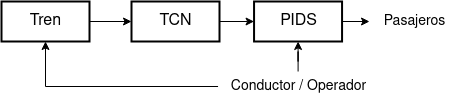
\includegraphics[width=0.66\textwidth]{./Figures/diagTrenTcnPids.png}
	\caption{Diagrama del sistema Tren-TCN-PIDS.}
	\label{fig:diagTrenTcnPids}
\end{figure}

La red TCN define una comunicación estándar usando dos buses jerárquicos llamados WTB (\textit{Wire Train Bus}) y MVB (\textit{Multifunction Vehicle Bus}). El sistema PIDS se interconecta al bus de datos MVB, como se indica en el diagrama de la figura \ref{fig:diagTcnPidsBuusesWtbMvb}.\\


\begin{figure}[ht]
	\centering
	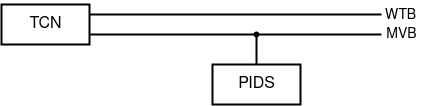
\includegraphics[width=0.66\textwidth]{./Figures/diagTcnPidsBusesWtbMvb.png}
	\caption{Diagrama de interconexión TCN-PIDS}
	\label{fig:diagTcnPidsBuusesWtbMvb}
\end{figure}

El sistema PIDS tiene un bus de comunicación propio a través de una red RS485. Uno de los componentes de esta red es el módulo SCU )descrito en la topolgía del PIDS del capítulo 2), al cual se conectan distintos dispositivos como los display led, los mapas de recorrido led, las cámaras y parlantes, tal como se indica en la figura 	\ref{fig:diagPidsScuDevices}.\\


\begin{figure}[ht]
	\centering
	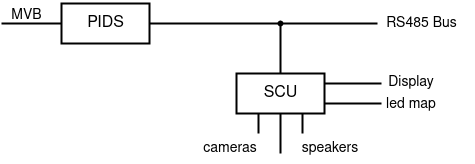
\includegraphics[width=0.66\textwidth]{./Figures/diagPidsScuDevices.png}
	\caption{Diagrama del módulo SCU en la red PIDS.}
	\label{fig:diagPidsScuDevices}
\end{figure}

Al módulo SCU se conectan las unidades IDU, que corresponden a los display led de salón. Cada unidad IDU contiene un controlador (\textit{driver}) y el arreglo de módulos de matriz led que conforman el display. En la figura \ref{fig:diagScuDriverDisplay} se representan estos bloques funcionales.\\


\begin{figure}[ht]
	\centering
	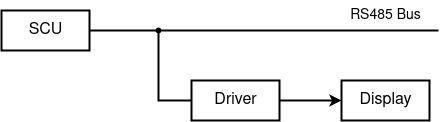
\includegraphics[width=0.66\textwidth]{./Figures/diagScuDriverDisplay.png}
	\caption{Diagrama de bloques del sistema SCU, placa de control y carteles led de salón.}
	\label{fig:diagScuDriverDisplay}
\end{figure}

El alcance del sistema desarrollado en este trabajo cubre la funcionalidad de este conjunto de bloques \textit{Driver + Display}, que en la nomenclatura del sistema PIDS existente corresponde a los módulos IDU. Existen dos unidades de estos módulos por cada salón o coche. Muchas de las formaciones de SOFSE disponen de siete coches, por lo que se tiene un mínimo de catorce unidades IDU (dos por salón), más dos displays externos adicionales para el frente y contrafrente del tren que indican las estaciones cabecera del recorrido. Esto resulta en un total de al menos dieciséis unidades de control de carteles de matriz led por cada tren. Teniendo en cuenta las formaciones operativas de las líneas Mitre, Sarmiento y Roca del Área Metropolitana de Buenos Aires (AMBA), se puede estimar alrededor de treinta trenes operando en simultáneo, lo que resulta en aproximadamente 500 unidades de carteles operando en vivo. El impacto que puede tener el aporte de este trabajo estará directamente relacionado con la operación de Trenes Argentinos, y puede contribuir a la extensión de la vida útil de los trenes.\\

\subsection{Diseño}
La propuesta de diseño busca cubrir las funcionalidades del bloque de control del display led. El display led es una unidad que se puede adquirir comercialmente. Sin embargo el driver para la red PIDS es una solución propietaria del fabricante y es la que se busca reemplazar con este desarrollo. En la figura \ref{fig:diagVistaReDisenhoEduCIAA} se presenta un diagrama de bloques del sistema de control propuesto. Este controlador usa comunicación serie a través de interfaces UART-RS485 y UART-USB. La UART (\textit{Universal Asynchronous Receiver Transmitter}) es un periférico del microcontrolador de la plataforma CIAA. La alimentación de la CIAA difiere de aquella existente en la red RS485 de Trenes Argentinos, por lo que también es necesario un bloque de conversión de tensión DC-DC para garantizar compatibilidad eléctrica. La comunicación con el display se realiza a través de un adaptador eléctrico, que consiste básicamente en un puerto de entrada-salida.\\


\begin{figure}[ht]
	\centering
	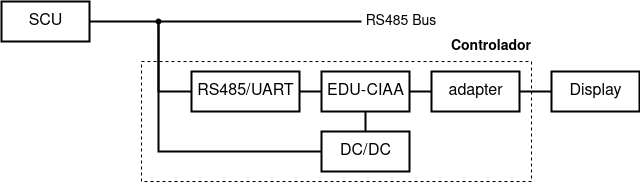
\includegraphics[width=1\textwidth]{./Figures/diagVistaReDisenhoEduCIAA.png}
	\caption{Diagrama de bloques del controlador propuesto.}
	\label{fig:diagVistaReDisenhoEduCIAA}
\end{figure}

A nivel lógico, el sistema que se propone consiste en cuatro objetos activos que interactúan entre sí, tal como se indica en la figura \ref{fig:diagVistaDisenho}. El prefijo '\underline{ao:}' señala que el bloque es un objeto activo. El objeto activo UART es el encargado de recibir e interpretar las tramas de datos que viajan por la red RS485 del bus de datos del SCU. El objeto activo Button es el control manual del operador para accionar el sistema. El objeto activo PIDS es una máquina de estados que representa el estado del tren, y contiene los mensajes y nombres de las estaciones. El objeto activo DisplayLed es el encargado de codificar los mensajes en el formato correspondiente a la matriz led del display.\\


\begin{figure}[ht]
	\centering
	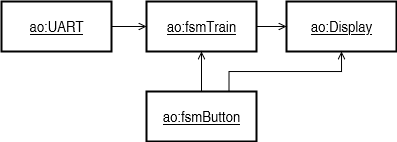
\includegraphics[width=1\textwidth]{./Figures/diagVistaDisenho.png}
	\caption{Vista estructural del sistema propuesto.}
	\label{fig:diagVistaDisenho}
\end{figure}



Esta vista estructural del sistema plantea la interacción entre componentes e indica su dependencia funcional. El diseño modular permite hacer cambios en los componentes de forma independiente. Por ejemplo, se podrían reemplazar los mensajes al pasajero en el objeto PIDS sin afectar el resto del sistema, o si fuera necesario cambiar el hardware de control, se podría reemplazar la lógica de control del display led modificando únicamente el objeto Displayled.\\


\section{Implementación}
En este trabajo se implementa un sistema embebido usando el lenguaje de programación C y el sistema operativo de tiempo real freeRTOS. La plataforma de hardware utilizada es la CIAA-EDU-NXP, que dispone de un microcontrolador LPC4337 de la companía NXP (\citep{NXPLPC4337}), con una arquitectura de 32 bits ARM Cortex-M4/M0. El firmware se desarrolló utilizando la \textit{SAPI} y el \textit{firmwarev3} \citep{firmwarev3} como capa de abstracción de hardware. Esta API es una interfaz para usar las funciones de la biblioteca CMSIS del fabricante del microcontrlador. Esta API es parte fundamental del proyecto CIAA.\\
 
En el diseño del sistema se desarrollaron plantillas para implementar patrones de software como máquinas de estado y objetos activos. La documentación, pruebas unitarias, mantenimiento y escalabilidad son los aspectos de calidad de software que se buscó satisfacer desde el diseño, y que se vieron facilitados con el uso de las plantillas. Los lineamientos y fragmentos de código relevantes de estas plantillas son descriptos en la sección de patrones de software. \\

La implementación de los objetos activos está descripta en la sección de componentes de sistema. Los atributos principales de la solución, las vistas de interacción entre componentes son parte de la documentación presentada. La implementación del controlador del diplay led tiene una sección a nivel de detalle para mayor comprensión. El firmware busca ser portable a aquellas versiones de hardware de display de matriz led compatibles con el conjunto de chips 74HC245, 74HC595 y 74HC138, o sistemas digitales equivalentes. \\



\subsection{Organización del código fuente}
La organización del código fuente que conforma el sistema embebido de este trabajo se detalla en el siguiente árbol de archivos:

\begin{lstlisting}[
	language=Bash, 
	backgroundcolor=\color{mygray},
	]
	
	
AppRTOS
|-- config.mk
|-- inc
|   |-- common.h
|   |-- displayled.h
|   |-- FreeRTOSConfig.h
|   |-- ISR_GPIO.h
|   |-- ISR_UART.h
|   |-- main.h
|   |-- modulePanelDisplay.h
|   |-- portmap.h
|   |-- statemachine_AB.h
|   |-- statemachine_button.h
|   |-- statemachine_displayled.h
|   |-- statemachine_PIDS.h
|   |-- statemachine_UART.h
|   `-- userTasks.h
|-- LICENSE.txt
`-- src
    |-- displayled.c
    |-- ISR_GPIO.c
    |-- ISR_UART.c
    |-- main.c
    |-- statemachine_AB.c
    |-- statemachine_button.c
    |-- statemachine_displayled.c
    |-- statemachine_PIDS.c
    |-- statemachine_UART.c
    `-- userTasks.c
\end{lstlisting}

Se pueden observar dos directorios principales: \textit{inc} y \textit{src}. En \textit{inc} se incluyen los archivos de encabezados y en \textit{src} los archivos de código ejecutable. Existe un archivo principal o \textit{main} que es el que instancia las secuencias de incialización, recursos y tareas del sistema operativo. Las tareas, que incluyen a los objetos activos y procesos del sistema, se implementan en los archivos \textit{userTasks}. Luego, para cada implementación de objeto activo existe una máquina de estados asociada en un archivo de encabezados (.h),  y un archivo ejecutable (.c) con el prefijo \textit{statemachine}. Finalmente los archivos con el prefijo \textit{ISR} corresponden a las rutinas de interrupción. Como cada máquina de estado utiliza recursos del sistema operativo, se ha creado un archivo \textit{common.h} que declara aquellos recursos como colas, \textit{handlers} y semáforos que se utilizan entre tareas para comunicación interprocesos.\\

Esta organización permite encapsulamiento y modularidad de los componentes del sistema. De esta manera se facilita el mantenimiento y, con el uso de las mismas reglas de diseño, se facilita la escalabilidad.\\

\subsection{Uso de recursos en RTOS}

En este desarrollo se utiliza freeRTOS, una versión en C de un \textit{kernel} de sistema operativo de tiempo real. La implementación se basa en la inclusión de los archivos de cabecera \textit{FreeRTOS.h} y \textit{FreeRTOSConfig.h}. Esta implementación ha sido validada en arquitecturas ARM Cortex-M4, en particular en la plataforma EDU-CIAA. 

En todos los casos que fue posible, se utilizaron semáforos, colas y \textit{mutex} para organizar y proteger el uso compartido de recursos. El caso de uso típico de \textit{mutex} es la interacción de distintas tareas con la misma interfaz UART-USB para imprimir mensajes por pantalla. En el código fuente de cada objeto implementado se utiliza la siguiente plantilla para proteger el recurso, evitando accesos múltiples y posibilidad de \textit{deadlock}:\\

\begin{lstlisting}[
	language=C, 
	backgroundcolor=\color{mygray},
	]
if (pdTRUE == xSemaphoreTake( xMutexUART, portMAX_DELAY)){
   vPrintString("Task AB is running.\r\n");
   xSemaphoreGive(xMutexUART);
}
\end{lstlisting}

Las colas, \textit{Queue}, se utilizan principalmente para comunicar eventos entre objetos activos. En todos los casos se referencian con \textit{handlers} usando el prefijo \textit{queueHandle} como nomenclatura. En el siguiente fragmento de código se muestra un ejemplo, exibiendo los mecanismos de control de errores utilizados. \\

\begin{lstlisting}[
	language=C, 
	backgroundcolor=\color{mygray},
	]
queueHandle_button = xQueueCreate(QUEUE_MAX_LENGTH, sizeof(eSystemEvent_button));
if (queueHandle_button == NULL){
    perror("Error creating queue");
    return 1;
}
\end{lstlisting}


Todas las tareas y recursos del sistema operativo se han protegido contra errores informando al usuario ante fallas en la instanciación, previas al inicio del \textit{scheduler} u orquestador.

\begin{lstlisting}[
	language=C, 
	backgroundcolor=\color{mygray},
	]
if( xTaskCreate( vTaskReadSerial, "Serial Comm reading task", 
    configMINIMAL_STACK_SIZE*4, NULL, tskIDLE_PRIORITY+2, &xTaskReadSerialHandler) 
    == pdFAIL ) {
    perror("Error creating task");
}
\end{lstlisting}

Se utilizan también punteros de tipo \textit{xTaskHandle} para referenciar las tareas del sistema operativo. Este tipo de referencias son de especial utilidad a la hora de eliminar tareas de forma dinámica en tiempo de ejecución. También es posible usar estas referencias para comunicación entre tareas.\\

El uso de \textit{timers} por software fue el preferido en aquellos casos que su uso facilita el mantenimiento, legibilidad y comprensión de la implementación. La plantilla desarrollada para la creación de \textit{timers} se presenta en el siguiente fragmento de código.

\begin{lstlisting}[
	language=C, 
	backgroundcolor=\color{mygray},
	]
void timerCallback_displayled(TimerHandle_t xTimerDisplayHandle){

   if (pdTRUE == xSemaphoreTake( xMutexUART, portMAX_DELAY)){
      printf("Timer display led is running.\r\n");
      xSemaphoreGive(xMutexUART);
   }

   eSystemEvent_displayled  displayled_timer_event = evDisplayled_timeout;
   
   if(xQueueSend(queueHandle_displayled, &displayled_timer_event, 0U)!=pdPASS){
         perror("Error sending data to the queueHandle_displayled\r\n");
   }
}

\end{lstlisting}

Se procuró tener especial cuidado de superposición o competición del reloj del sistema operativo entre tareas. Distintos componentes pueden tener requisitos temporales que compiten entre si por prioridad del orquestador. Se verá en detalle la implementación del display led como ejemplo que puede competir con el arribo de mensajes por la interfaz UART.\\

Las rutinas de interrupción por hardware, o \textit{ISR}, se utilizan cuando se requiere respuesta inmediata. Por ejemplo, al accionar manualmente un interruptor o bien al recibir mensajes o señales eléctricas desde el bus de datos del tren. La implementación elegida para el uso de interrupciones se representa con en el diagrama de secuencia de la figura \ref{fig:ISR}. \\

\begin{figure}[ht]
	\centering
	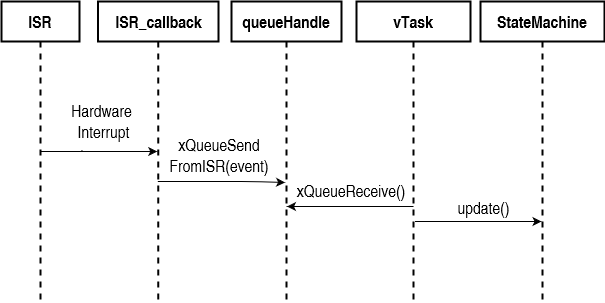
\includegraphics[width=1\textwidth]{./Figures/ISRcallback.png}
	\caption{Diagrama de secuencia que representa la interacción entre componentes del sistema operativo cuando se dispara una interrupción o ISR.}
	\label{fig:ISR}
\end{figure}

El recurso de hardware que genera interrupciones (ISR) llama a una función \textit{callback} (\textit{ISR callback}), que sólo se encarga de entregar un mensaje de evento al sistema. Esta función no tiene lógica implementada, sólo avisa al sistema que hay una interrupción que atender. El evento se comunica a través de una cola, recurso elegido como interfaz de mensajes de los objetos activos. La cola es atendida por una tarea de sistema (\textit{vTask}) que resuelve el código de ejecución. Esta tarea normalmente implementa un objeto activo que actualiza una máquina de estado.\\

Si bien puede llamar la atención la complejidad del mecanismo de atención de una interrupción, este patrón basado en objeto activo permite desacoplar la invocación y la ejecución de una máquina de estados. El objeto activo es una técnica de concurrencia muy utilizada por la ventaja de separar en hilos independientes (\textit{threads}) la invocación de funciones (eventos) de las funciones de ejecución. Con este mecanismo aparece la posibilidad de atender múltiples eventos en simultáneo, sin esperar a que se procese cada evento secuencialmente. Se logra paralelismo, atomicidad en la función que atiende la interrupción, muy baja latencia, y consistencia con en el uso de objetos activos bajo los lineamientos de la arquitectura orientada a eventos.\\


Por último se menciona el uso de memoria dinámica. El sistema tiene una interfaz de comunicación UART que a priori recibirá mensajes de largo variable y desconocido. Por lo tanto, el uso de \textit{buffers} dinámicos para el almacenamiento y procesamiento de datos fue el mecanismo preferido. Para utilizar memoria dinámica se usan las funciones \textit{memset()}, \textit{pvPortMalloc()}, \textit{memcpy()} y \textit{vPortFree()}, a través de dos instancias de ejecución: una de recepción y almacenamiento de datos, y otra de ejecución y liberación de memoria. En el siguiente fragmento de código se explica este uso de funciones con dos tareas: \textit{reader} y \textit{writer}.


\begin{lstlisting}[
	language=C, 
	backgroundcolor=\color{mygray},
	]
void vTaskReader(void *parameters) {
   // Clear whole buffer
   memset(buf, 0, buf_len);
   // Loop forever
   while (true) {
   // Read from UART
      uint8_t c_data=0;
      if (uartReadByte( UART_USB, &c_data ) == true ){
      // Store to buffer if not over buffer limit  
         if (idx < buf_len - 1){
            buf[idx] = c_data;
            idx++;
         }
         // Create a message ending string with null
         if (c_data == '\n') {
            buf[idx - 1] = '\0';
            // Allocate memory and copy message. 
            if (msg_flag == 0) {
               msg_ptr = (char *)pvPortMalloc(idx * sizeof(char));
               if (msg_ptr==NULL){
                  if (pdTRUE == xSemaphoreTake( xMutexUART, portMAX_DELAY)){
                     printf("Buffer out of memory\r\n");
                     xSemaphoreGive(xMutexUART);
                  }
               }
               // Copy message
               memcpy(msg_ptr, buf, idx);
               // Notify other task that message is ready
               msg_flag = 1;
            }
            // Reset buffer and index
            memset(buf, 0, buf_len);
            idx = 0;
         }
      }
   }
}     

void vTaskWriter(void *parameters) {
   if (uart_msg_flag == true) {
      // Print the message in the buffer 
      if (pdTRUE == xSemaphoreTake( xMutexUART, portMAX_DELAY)){
        printf("%s\r\n", uart_msg_ptr);
        xSemaphoreGive(xMutexUART);
      }
      // Free the memory block  
      vPortFree(uart_msg_ptr);  
      uart_msg_ptr  = NULL;
   }
}

\end{lstlisting}

Como se puede observar, cuando se recibe un caracter por la interfaz UART se copia el mismo en el \textit{buffer}, siempre y cuando no esté lleno. Cuando el \textit{buffer} se completa, se pide memoria y se copia el mensaje usando un puntero al bloque de memoria asignado. Luego, la tarea de ejecución lee el mensaje de ese puntero a memoria, o bien lo procesa para invocar otra función.\\


\subsection{Patrones de software}
En este desarrollo se ha hecho uso extensivo de los patrones máquina de estado, objeto activo, \textit{pipeline}, observar y reaccionar, y superciclo. Se presenta en detalle el formato de plantillas desarrollado en C para freeRTOS para los patrones de máquinas de estado y de objeto activo. \\

\subsubsection{Máquinas de estado}
El desarrollo de la arquitectura orientada a eventos propuesta se basa en la interacción de máquinas de estado usando objetos activos. En este trabajo, las máquinas de estado se implementan sistemáticamente en C con un procedimiento paso a paso que se describe a continuación, usando como ejemplo una máquina de dos estados A y B que salta de un estado a otro por un evento temporal (\textit{evTimeout}):

\begin{enumerate}
\item Representación de los estados y eventos con diagrama de estados.
\begin{figure}[ht]
	\centering
	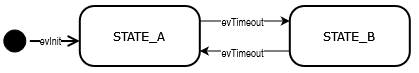
\includegraphics[width=0.66\textwidth]{./Figures/statemachineAB.png}
	\caption{Diagrama de la máquina de estados AB ejemplo.}
	\label{fig:fsmAB}
\end{figure}

\item Definición de los estados, usando tipo enumerativo definido con el prefijo \textit{eSystemState}:

\begin{lstlisting}[
	language=C, 
	backgroundcolor=\color{mygray},
	]
typedef enum{
    
    STATE_INIT,
	STATE_A,
	STATE_B

} eSystemState;
\end{lstlisting}

\item Definición de los eventos. Los eventos representan transiciones entre estados con un tipo enumerativo definido con el prefijo \textit{eSystemEvent}:

\begin{lstlisting}[
	language=C, 
	backgroundcolor=\color{mygray},
	]
typedef enum{

	evInit,
	evTimeout

} eSystemEvent;
\end{lstlisting}

\item Definición de un tipo puntero a función usando el prefijo \textit{*pfEventHandler()} para designar los handlers específicos:

\begin{lstlisting}[
	language=C, 
	backgroundcolor=\color{mygray},
	]
typedef eSystemState (*pfEventHandler)(void);
\end{lstlisting}

\item Definición de una estructura para la máquina de estados definiendo un tipo \textit{sStateMachine}. Esta estructura debe incluir una variable estado (\textit{eSystemState}), una variable evento (\textit{eSystemEvent}) y un puntero a función (\textit{pfEventHandler}). El puntero a función será una instancia de \textit{handler} específico que maneje las transiciones entre estados. 

\begin{lstlisting}[
	language=C, 
	backgroundcolor=\color{mygray},
	]
typedef struct{

	eSystemState  	fsmState;
	eSystemEvent  	fsmEvent;
	pfEventHandler	fsmHandler;

} sStateMachine;
\end{lstlisting}

\item Definición de los \textit{handlers} a implementar para el manejo de ejecución y transiciones entre estados.

\begin{lstlisting}[
	language=C, 
	backgroundcolor=\color{mygray},
	]
eSystemState 	InitHandler(void);
eSystemState 	AHandler(void);
eSystemState 	BHandler(void);
\end{lstlisting}

\item Instanciación de la máquina de estados como un arreglo de estructuras usando el prefijo \textit{sStateMachine\_}. Para el ejemplo de la máquina AB, la instancia de arreglo de estructuras sería la siguiente:

\begin{lstlisting}[
	language=C, 
	backgroundcolor=\color{mygray},
	]
sStateMachine_AB fsmMachineAB [] = 
{
	{STATE_INIT_AB, evInit_AB, InitHandler_AB},
	{STATE_A, evTimeout, AHandler},
	{STATE_B, evTimeout, BHandler}
};
\end{lstlisting}

En esta definición habrá un \textit{handler} en el momento de inicialización (\textit{initHandler}) y  un \textit{handler} específico para cada estado.

\item Escribir el código ejecutable de los \textit{handlers}. Una implementación a modo de ejemplo se presenta en el siguiente fragmento de código:

\begin{lstlisting}[
	language=C, 
	backgroundcolor=\color{mygray},
	]
eSystemState 	InitHandler(void){ 
	printf("State Machine Init...\n");
	return STATE_A; 
}

eSystemState 	AHandler(void){ 
	printf("State Machine State A\n");
	return STATE_B; 
}

eSystemState 	BHandler(void){ 
	printf("State Machine State B\n");
	return STATE_A; 
}
\end{lstlisting}
\end{enumerate}


Se debe notar que para este ejemplo cada transición de estados se ejecutará por el evento \textit{evTimeout}. La máquina inicia y se define en el estado STATE\_A y luego alterna entre \textit{STATE\_A} y \textit{STATE\_B} por cada evento de timeout.

De esta manera, queda desacoplada la implentación de los \textit{handlers} del resto de la estructura de la máquina de estados, logrando portabilidad, escala y modularidad. Los \textit{handlers} serán funciones que se implementan con el sufijo \textit{Handler()} y que por definición tienen un solo argumento de tipo \textit{void}.

Con esta técnica de desacoplamiento, se implementan dos archivos por cada máquina de estado : uno de encabezados (\textit{stateMachine.h}) con las definiciones, y otro con la implementación (\textit{stateMachine.c}) de los handlers.




\subsubsection{Objeto activo}
	
Los objetos activos se implementan en esta aplicación como tareas de freeRTOS, usando dos superciclos anidados de tipo \textit{while(true)}, tal como se muestra en el siguiente fragmento de código: 

\begin{lstlisting}[
	language=C, 
	backgroundcolor=\color{mygray},
	]
void vTaskAB(void *xTimerHandle)
{
   (void)xTimerHandle;

   // Task successful creation message
   if (pdTRUE == xSemaphoreTake( xMutexUART, portMAX_DELAY)){
      printf("Task AB is running.\r\n");
      xSemaphoreGive(xMutexUART);
   }

   while(true){
      
      // State machine init
      eSystemEvent_AB newEvent	=	evInit_AB;
      eSystemState_AB nextState	=	STATE_INIT_AB;
      fsmMachineAB[nextState].fsmEvent = newEvent; 
      nextState = (*fsmMachineAB[nextState].fsmHandler)();

      // Active object
      while(true){
        if( pdPASS == xQueueReceive(queueHandle_AB, &newEvent, portMAX_DELAY)){
            fsmMachineAB[nextState].fsmEvent = newEvent; 
            nextState = (*fsmMachineAB[nextState].fsmHandler)();
         }
      }
   }
}
\end{lstlisting}

Notar que el primer ciclo \textit{while()} es el que corresponde al funcionamiento normal de una tarea o proceso de RTOS. En este caso, es el encargado de inicializar la máquina de estados asociada al objeto activo. El ciclo \textit{while()} de la línea 20 se encarga de bloquear la tarea hasta que se reciba un evento por la interfaz (cola de eventos). La interfaz del objeto activo es una cola FIFO (\textit{First In First Out}) con la función de sistema \textit{xQueueReceive() }(línea 21). Si se recibe un evento, entonces se actualiza el estado de la máquina instanciando el handler que corresponda, como se observa en la línea 25. El diagrama de la figura \ref{fig:AOfsmAB} representa el objeto activo detallado. 

\begin{figure}[ht]
	\centering
	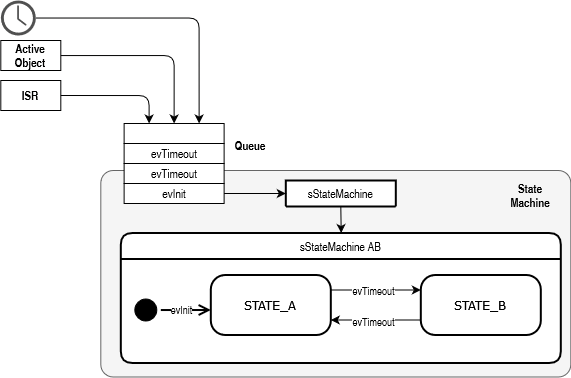
\includegraphics[width=0.85\textwidth]{./Figures/AOstatemachineAB.png}
	\caption{Diagrama del objeto activo de la máquina de estados AB ejemplo.}
	\label{fig:AOfsmAB}
\end{figure}

Para este ejemplo, la tarea de sistema recibe una referencia a un timer (\textit{xTimerHandle}) que genera eventos de \textit{timeout} y los encola en la interfaz del objeto activo (\textit{Queue}). Con la misma interfaz, los eventos también podrían ser generados por otros objetos activos, o por rutinas de interrupción. Los mensajes en cola los recibe  la tarea de sistema que actualiza la máquina de estados (\textit{vTaskAB}).\\

\subsection{Componentes del sistema}

En esta sección se describen los componentes principales de la solución representada con el diagrama estructural de la figura \ref{fig:diagVistaDisenho}. En la figura \ref{fig:diagramaSecuenciaSistema} se presentan las interacciones entre componentes en forma de secuencia para los distintos casos de uso. Los cuatro objetos activos utilizados son:\\
\begin{itemize}
\item \textbf{UART}: objeto activo que sirve de interfaz de comunicación con la red RS485 del sistema PIDS. Se encarga de recibir los mensajes de la red, identificarlos y enviarlos al objeto PIDS.
\item \textbf{PIDS}: objeto activo que contiene la lógica de procesamiento de señales del tren, los mensajes que se visualizan en pantalla y los trayectos disponibles. 
\item \textbf{displayled}: objeto activo responsable de codificar los mensajes que vienen del PIDS para ser visualizados en un display de matriz led.
\item \textbf{Button}: objeto activo responsable de recibir accionamientos manuales del conductor del tren.
\end{itemize}

\begin{figure}[ht]
	\centering
	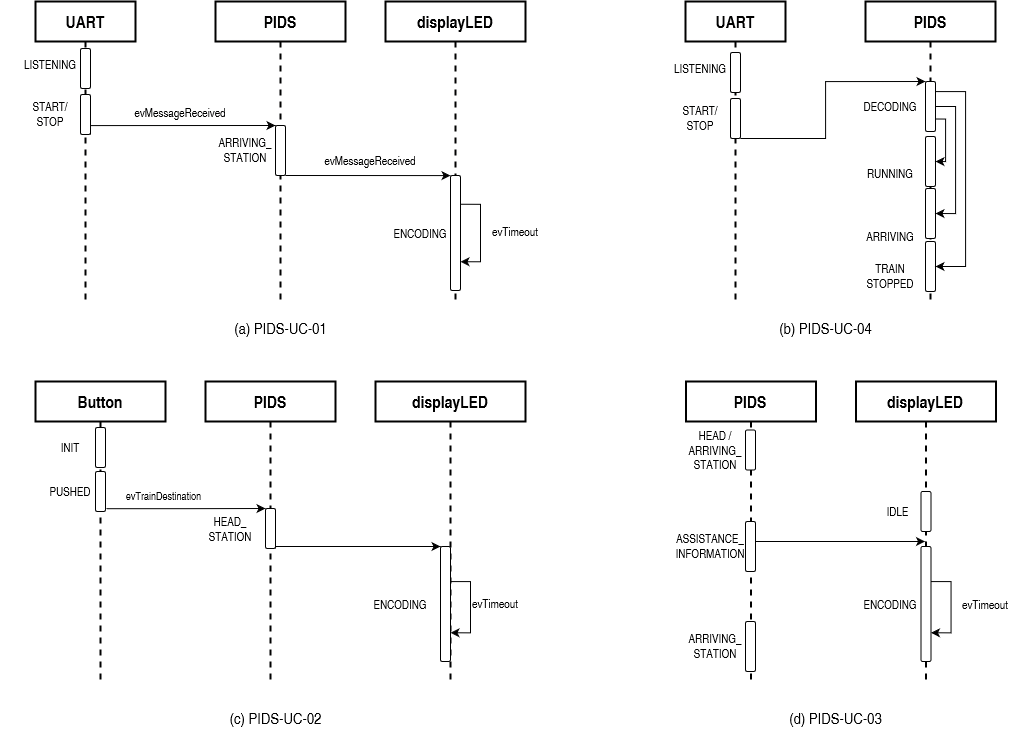
\includegraphics[width=1\textwidth]{../Figures/secuenciasSistema.png}
	\caption{(a)caso de uso de visualización de estación; (b) caso de uso de receptor de tramas;(c) caso de uso de elección de destino por accionamiento del conductor;(d) caso de uso de visualización de información de asistencia.}
	\label{fig:diagramaSecuenciaSistema}
\end{figure}


%La organización del orquestador del sistema operativo se representa con el diagrama temporal de la figura \ref{fig:diagramasTemporales}. La base de este diagrama es el orden de prioridades de las tareas de objetos activos, los timers y los handlers de interrupciones que manejan los periféricos de hardware.\\

\subsubsection{UART}

 Este tipo de interfaz suele ser común en numerosas aplicaciones y abundan ejemplos utilizados para leer y escribir desde y hacia un periférico UART. El caso trivial es una aplicación \"eco\": todo lo que se recibe por la UART se vuelve a escribir y enviar por la UART. Sin embargo, la aplicación específica determina la lógica de procesamiento de mensajes. Por ejemplo, si se recibe un caracter determinado, entonces se activa tal objeto; si se genera un evento en tal otro objeto, entonces se envía un mensaje de aviso. \\

En el sistema desarrollado, la UART es la interfaz de comunicación con el resto de la red PIDS. Esta debe procesar eventos que indican aceleración y desaceleración del tren. Los eventos se reciben codificados en tramas con formato específico, que a priori carecen de documentación. Como se verá en la sección de ensayos, se ha observado que las tramas normalmente tienen un encabezado (\textit{header}), una carga de datos (\textit{payload}), y un final de trama (\textit{trailer}). Sin embargo, también se ha observado que los mensajes del tren pueden tener largo variable. El diseño de este componente se representa con el diagrama de la figura \ref{fig:diagfsmUART}.\\


\begin{figure}[ht]
	\centering
	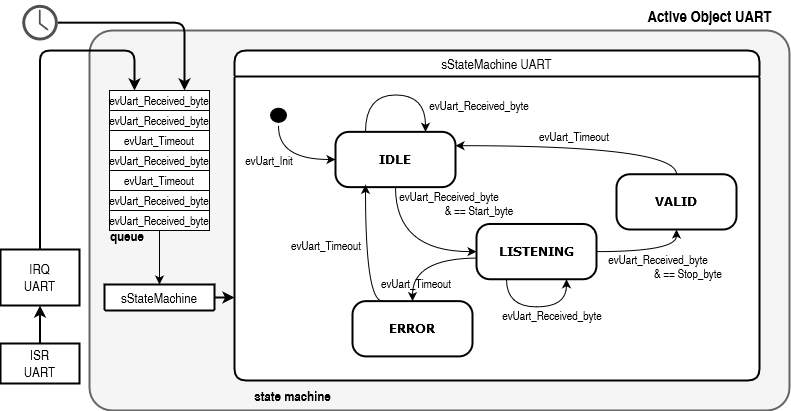
\includegraphics[width=1\textwidth]{./Figures/fsmUART3.png}
	\caption{Diagrama del objeto activo UART implementado.}
	\label{fig:diagfsmUART}
\end{figure}

El periférico UART es un componente de bajo nivel del microcontrolador que admite el control por interrupciones (ISR). Cada byte entrante genera una interrupción y de inmediato el \textit{handler} \textit{IRQ\_UART} envía un mensaje de actualización al objeto activo. Los eventos admitidos son:
\begin{itemize}
\item \textit{evUart\_Received\_byte} para la recepción de un byte de datos; 
\item \textit{evUart\_Timeout}, generado por un timer específico de control.\\
\end{itemize} 

La máquina de estados admite cuatro estados distintos:
\begin{itemize}
\item \textit{IDLE}: estado inicial y de reposo.
\item \textit{LISTENING}: estado generado al recibir el Header o inicio de trama.
\item \textit{VALID}: estado generado al completar un mensaje con el Trailer o final de trama.
\item \textit{ERROR}: estado alcanzado una vez generado un timeout en el estado listening.
\end{itemize}

El estado \textit{LISTENING} es el \textit{core} de la máquina de estados. El \textit{handler} de ejecución permite guardar en memoria dinámica el contenido de un mensaje de largo variable una vez que se recibe un byte de inicio de trama.  El mensaje se completa cuando se recibe un byte de final de trama, que genera mediante \textit{timeout} el evento de transición al estado \textit{Valid}. La lógica que se plantea con este diseño es que, una vez validada una trama de datos, se genere un evento de actualización hacia el componente externo PIDS. De esta manera, se desarrolló un componente UART con flexibilidad, que permite cambiar los bytes de \textit{header} y \textit{trailer} y admite un \textit{buffer} de largo variable usando memoria dinámica. \\

\subsubsection{Display led}

En esta sección se describe la solución implementada para controlar carteles de matriz led. La estructura de control, el conjunto de chips compatibles, el uso y posible reutilización en otros sistemas se presenta con diagramas y detalles de código fuente. \\

Los carteles led utilizados en este trabajo se basan en una tecnología de microcontrolador (MCU) y sistema digital. El MCU genera las señales de control y el sistema digital se encarga de codificar y multiplexar los datos binarios en señales eléctricas, para prender los leds del cartel de forma ordenada. Los carteles se componen de módulos matriciales de 8x8 leds, es decir, 8 filas de 8 leds por fila cada módulo. Los arreglos de módulos forman paneles, y los arreglos de paneles forman carteles. Los módulos se pueden controlar enviando pulsos de tensión a las filas y columnas. Sin embargo, si se quisiera controlar varios módulos de matriz led en simultáneo, la cantidad de señales a priori podría ser proporcional al número total de leds. El sistema digital expone una solución para que los paneles, como arreglos de módulos, puedan ser direccionados por un grupo de tres o cuatro señales de control usando técnicas de multiplexación y registros de desplazamiento, o \textit{Shift Registers}, como se describe a continuación. \\


\begin{figure}[ht]
	\centering
	\includegraphics[width=1\textwidth]{./Figures/diagDriverled.png}
	\caption{Diagrama de bloques del controlador de los carteles de matriz led utilizados en esta implementación.}
	\label{fig:diagDriverled}
\end{figure}

En la figura \ref{fig:diagDriverled} se presenta un diagrama de bloques del sistema digital de control para carteles de matriz led basados en el \textit{chipset} 74HC245, 74HC595 y 74HC138. Se pueden distinguir los siguientes bloques:

\begin{itemize}
\item \textit{MCU}: se encarga de generar y transmitir las señales del sistema a través del conector de entrada.
\item \textit{input connector}: conector de pines para señales de entrada (\textit{Data, Clock, Latch}) provenientes del MCU.
\item \textit{output connector}: conector de pines para señales de salida, para interconexión en serie con otro cartel.
\item \textit{Buffer}: adaptador de nivel de la señal de tensión y derivador a izquierda o derecha de la placa física.
\item \textit{Shift Registers}: registros de desplazamiento para enviar datos binarios a las columnas de los paneles.
\item \textit{Deco}: doble decodificador 3x8 para energizar secuencialmente las filas de los paneles.
\item \textit{MOSFET Array}: \textit{driver} de corriente para el encendido de filas de los paneles.
\item \textit{Led dot matrix array}: el cartel de matriz led propiamente dicho.
\end{itemize}

%El funcionamiento del circuito sigue básicamente un control ordenado de filas y columnas. 
El funcionamiento para visualizar mensajes en el cartel es el siguiente. Se debe transformar el mensaje a visualizar como texto plano, y luego codificarlo en una matriz de unos y ceros que tenga las dimensiones del cartel. Por ejemplo, en un arreglo de 16 módulos 8x8, se podrían enviar mensajes de hasta 16 caracteres, usando un módulo para cada caracter. Para codificar cada caracter hace falta un diccionario que permita transformar cada caracter en una matriz de 8x8 datos binarios. En la figura \ref{fig:dataPipeline} se muestra un ejemplo con la letra 'H' codificada por la función f1, y se presenta la implementación desarrollada usando el patrón \textit{pipeline} (f1 y f2) para preprocesar mensajes de texto en datos binarios compatibles con el formato de carteles de matriz led.

\begin{figure}[htbp]
	\centering
	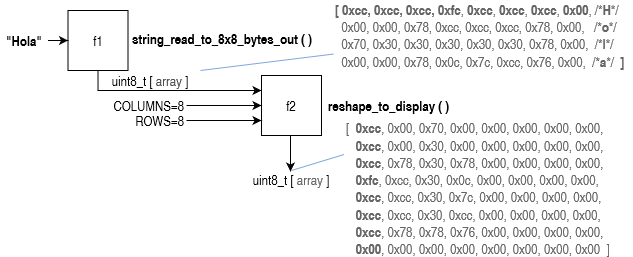
\includegraphics[width=1\textwidth]{./Figures/dataPipeline.png}
	\caption{Procesamiento de datos para codificar mensajes.}
	\label{fig:dataPipeline}
\end{figure}

Una vez disponibles los datos binarios del mensaje en formato de filas y columnas, las señales de control (\textit{data}, \textit{clock}, \textit{latch}, \textit{deco}) se generan en el MCU y se transmiten al circuito eléctrico del display led usando el conector de entrada. Estas señales se direccionan eléctricamente usando \textit{buffers} 74HC245D, que además ratifican el nivel lógico de tensión por ejemplo a 5 Volt. A la izquierda se transmiten las señales \textit{Data}, \textit{Clock} y \textit{Latch}, y a la derecha las señales para que los decodificadores 74HC138 enciendan hasta 16 salidas secuencialmente. Siguiendo la señal de reloj como base, se envían bit a bit  y usando el arreglo de \textit{Shift Registers} para enviar los datos de módulo en módulo. Los datos se envían como números hexadecimales en la señal de \textit{data}, y los registros de desplazamiento tienen 8 salidas las columnas de cada módulo. Los registros de desplazamiento son los encargados de transmitir bit a bit los datos de las columnas de. Una vez enviados todos los datos de una fila, se envía un pulso como señal de \textit{latch} y se energiza la fila completa. Luego se repite la operación fila a fila, escaneando todo el cartel a través de las señales del \textit{Deco}, energizando cada fila a través de un arreglo de transistores \textit{MOSFET} que mantienen la corriente necesaria para encender los leds. Este encendido por fila sucede durante un período de tiempo tal que toda la pantalla se pueda energizar en el orden de 20 a 50 veces por segundo, para formar una imagen continua vista por el ojo humano.\\

 
 Para armar carteles más grandes, se suele enchufar el conector de salida de un cartel con el conector de entrada de otro, logrando conexiones en serie entre paneles. De esta manera, un sólo panel se conecta al MCU y el resto sigue una conexión en cascada, usando el mismo grupo de señales.


\begin{figure}[ht]
	\centering
	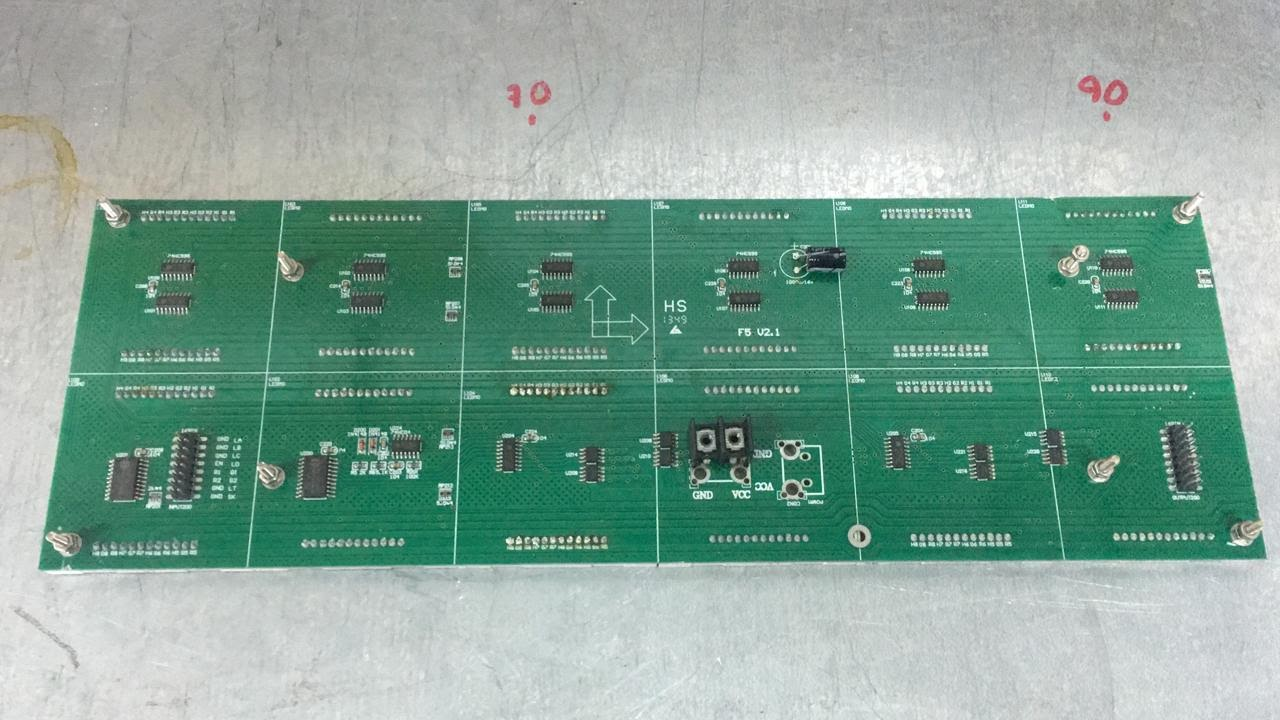
\includegraphics[width=1\textwidth]{./Figures/cartel2x6.jpeg}
	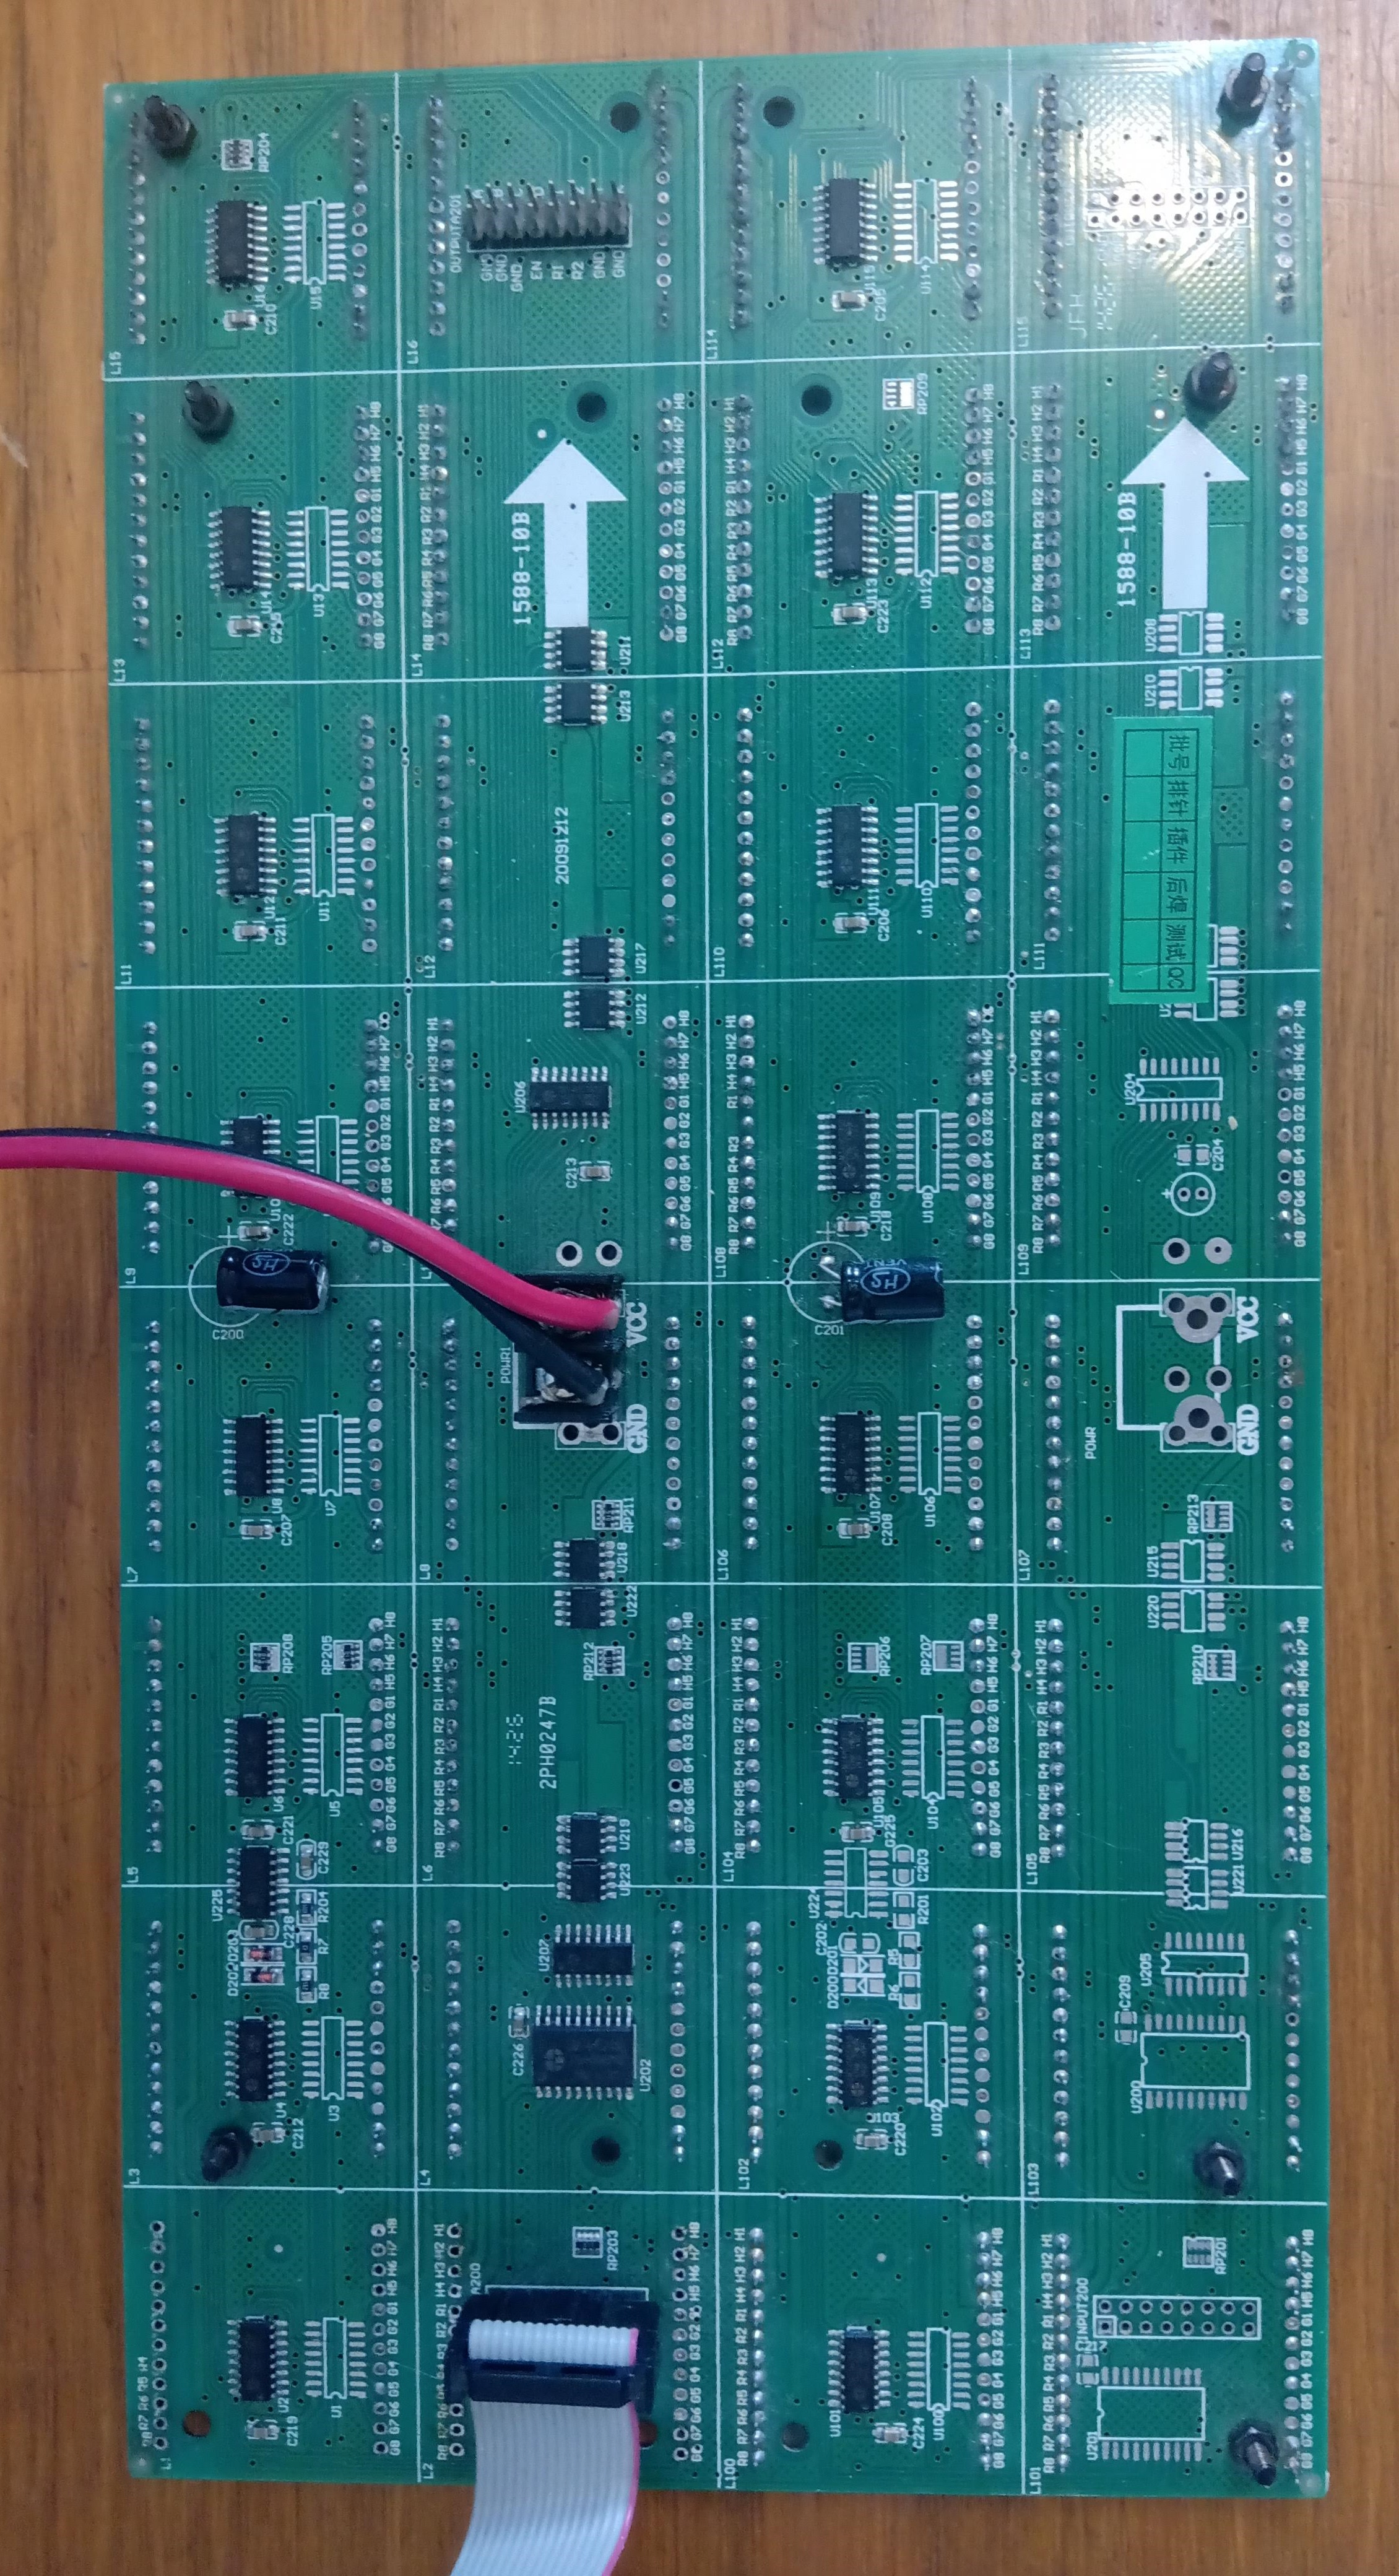
\includegraphics[width=0.75\textwidth, angle=270]{./Figures/cartel4x8.jpg}\\
	\includegraphics[width=1\textwidth]{./Figures/cartelledON.jpg}\\
	\caption{Fotografías de placas de control de los carteles de matriz led: (a) placa de 2x6 módulos; (b) placa de 4x8 módulos; (c) vista posterior de la placa de 4x8.}
	\label{fig:picsDriverled}
\end{figure}

En el circuito esquemático de la figura \ref{fig:schDriverled} se presenta el detalle de conexiones eléctricas entre bloques. Se puede observar que a la salida del conector de datos (CONN 2x8) hay dos buffers de la serie 74HC245D que direccionan las señales eléctricas a izquierda y derecha del arreglo de matrices led. A izquierda viajan las señales SER(data), SRCLK (Clock) y XXX (latch) al arreglo de Shift Registers de la serie 74HC595. Por la derecha se maneja la habilitación secuencial de las filas a través de un arreglo de decodificadores 3x8 de la serie 74HC138. Cada salida de los decodificadores se conecta a un driver de corriente en arreglo de transistores MOSFET FDS4953. Estos decodificadores cableados adecuadamente permiten manejar las 32 señales de un cartel de 4x8 módulos led. \\
%
%
%\begin{figure}[ht]
%	\centering
%	%\includepdf[pages={1}, angle=90]{./Figures/output.driverled.pdf}
%	\includegraphics[width=1.66\textwidth, angle=90]{./Figures/output.driverled.pdf}
%	\caption{Circuito esquemático de la placa controladora de los carteles de matriz led.}
%	\label{fig:schDriverled}
%\end{figure}

La pieza de software desarrollada para el control del display led es un objeto activo consistente con el resto del sistema. El diagrama de la máquina de estados asociada se presenta en la figura \ref{fig:fsmDisplayled}. Se pueden distinguir tres estados, cada uno con un handler asociado. En el siguiente fragmento de código se presenta la especificación de la máquina de estados del display led. \\\\

\begin{figure}[htbp]
	\centering
	\includegraphics[width=0.66\textwidth]{./Figures/FSMdisplayled.png}
	\caption{Diagrama de estados para la máquina de estados del display led.}
	\label{fig:fsmDisplayled}
\end{figure}



\begin{lstlisting}[
	language=C, 
	backgroundcolor=\color{mygray},
	caption=	{Display led state machine definition},
	captionpos=b]
sStateMachine_displayled fsmDisplayled[] = 
{
    {STATE_DISPLAYLED_INIT, evDisplayled_init, displayled_initHandler},
    {STATE_DISPLAYLED_IDLE, evDisplayled_msg_received, displayled_idleHandler},
    {STATE_DISPLAYLED_PROCESSING, evDisplayled_timeout, displayled_procHandler},
    {STATE_DISPLAYLED_ENCODING, evDisplayled_timeout, displayled_dataHandler}
};
\end{lstlisting}
\label{code:fsmDisplay}



\begin{lstlisting}[
	language=C, 
	backgroundcolor=\color{mygray},
	caption=	{Código fuente del handler de procesamiento del display led.},
	captionpos=b]

eSystemState_displayled     displayled_procHandler(void){

    char *str1=messages[displayled_msg_idx];

    uint8_t str1_len=strlen(str1);
    uint8_t buffer_size=str1_len*CHAR_LENGTH;
    uint8_t buffer[buffer_size];

    string_read_to_8x8_bytes_out(str1,str1_len,buffer);

    int n=CHAR_LENGTH; 
    int m=str1_len;
    int p=DISPLAYLED_ROWS;
    int q=DISPLAYLED_COLS;

    int displayled_size = p*q;

    uint8_t B[displayled_size];
    for(int i=0; i<displayled_size;i++)
    B[i]=0;

    reshape_to_display(buffer, displayled_buffer, buffer_size, displayled_size);

    displayled_msg_idx++;
    displayled_msg_idx%=MESSAGES_TOTAL_NUMBER;
    displayled_msg_flag=0;

    return STATE_DISPLAYLED_ENCODING;
}

\end{lstlisting}

El estado 'STATE\_DISPLAYLED\_PROCESSING' ejecuta el handler  'displayled\_procHandler()' encargado de recibir mensajes externos en formato string (char*). Este implementa un pipeline de procesamiento para transformar strings en matrices de enteros de 8 bits.

%\begin{figure}[ht]
%	\centering
%	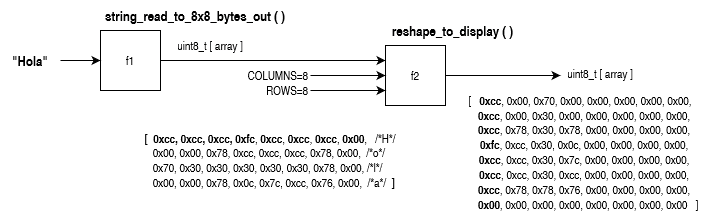
\includegraphics[width=1\textwidth]{./Figures/pipelineDataEncoding.png}
%	\caption{Lógica de procesamiento de datos para visualizar en el display.}
%	\label{fig:displayDataLogic}
%\end{figure}


\begin{lstlisting}[
	language=C, 
	backgroundcolor=\color{mygray},
	caption=	{Código fuente del handler de encoding del display led.},
	captionpos=b]
	
eSystemState_displayled     displayled_dataHandler(void){

    uint8_t data_8b;
    bool_t  value;

    displayled_timer_cnt--;
    if(!displayled_timer_cnt){
        displayled_msg_flag=0;
        return STATE_DISPLAYLED_IDLE;
    };    

    for(int i=0; i<displayled_size; i++){
        
        data_8b = displayled_buffer[i];
        
        for(int j=0; j<8; j++){
            
            // displayled_data 
            value = (((data_8b << j ) & 0x80 ) == 0) ? 1 : 0;
            printf("%d",value);
            gpioWrite(displayled_panel_1, value);
            gpioWrite(displayled_panel_2, value);
            
            // displayled_clock 
            gpioWrite(displayled_clk, ON);
            gpioWrite(displayled_clk, OFF);
        }
        
        if(i%DISPLAYLED_COLS==0){

            // displayled_latch 
            printf("\r\n");
            gpioWrite(displayled_latch, ON);
            gpioWrite(displayled_latch, OFF);
            
            // displayled_row_scanning
            displayled_deco_cnt++;
            displayled_deco_cnt%=DISPLAYLED_ROWS;
            if((displayled_deco_cnt%1)==0){ 
            		gpioToggle(displayled_deco_A0); }
            if((displayled_deco_cnt%2)==0){ 
            		gpioToggle(displayled_deco_A1); }
            if((displayled_deco_cnt%4)==0){ 
            		gpioToggle(displayled_deco_A2); }
            if((displayled_deco_cnt%8)==0){ 
            		gpioToggle(displayled_deco_A3); }
        }
    }
    
    return STATE_DISPLAYLED_ENCODING;
}

\end{lstlisting}
